\documentclass[11pt]{article}
\pagestyle{plain}
\usepackage{latexsym,exscale,amsfonts,amsmath,amssymb,array,graphicx}
\usepackage{color}
\usepackage[colorlinks]{hyperref}
\setlength{\topmargin}{-2.3cm}
\setlength{\textheight}{23.8cm}
\setlength{\oddsidemargin}{-0.5cm}
\setlength{\textwidth}{17cm}
\setlength{\parindent}{0cm}
\setlength{\parskip}{.4cm}
\newcommand{\totaldiffx}{\frac{d}{dx}}
\newcommand{\pardiffx}{\frac{\partial}{\partial x}}
\newcommand{\luft}{\:\!}

\usepackage{graphicx}
\usepackage[latin1]{inputenc}
\usepackage{mathpazo}
\usepackage[T1]{fontenc}
\usepackage[comma,numbers,sort&compress]{natbib}


\begin{document}
\begin{center}
\large \bf Computational Astrophysics \rm \\
2019\\
{\small Solution Exercise 6.2}
\end{center}


{\bf 6.2 Number Density of Electrons in an Astrophysical Environment}

In high temperature astrophysical environments ($T \gtrsim 10^9\,\mathrm{K} \sim
80\,\mathrm{keV}$), the reaction 
\begin{equation}
\gamma \leftrightarrow e^- + e^+
\end{equation}
comes into equilibrium. We will assume the
limit of $k_B T = 20\,\mathrm{MeV} \gg m_ec^2$, when the electrons
become relativistic, i.e. $E_{e^-} \sim E_{e^+} = pc$ where $p$ is the
momentum of the electrons and positrons and $c$ is the speed of light.

In such an environment, the number density of electrons/positrons is given by
\begin{equation}
n_{e^\pm} = {2 \over (2\pi\hbar)^3}\int { d^3\vec{p} \over
  e^{\beta c p} + 1} = {8\pi \over (2\pi\hbar)^3}\int_0^\infty {p^2 dp \over
  e^{\beta c p} + 1},
\end{equation}
where $\beta = 1/(k_B T)$. Making the substitution of $x= \beta p c$ to make the integral
dimensionless, we obtain

\begin{equation}
n_{e^\pm}  =  {8\pi (k_BT)^3 \over (2\pi\hbar
  c)^3}\int_0^\infty  \frac{x^2 dx}{e^{x} + 1}. \label{eq:ElectronDensity}
\end{equation}
 
 Note that in this deduction we have considered that the chemical potential of the
electrons (and  positrons) is 0.

\begin{enumerate}
\item[(a)] Use any of the presented integration methods to determine what
  is the total number density of electrons in this environment. Try different conditions to ensure convergence. 

\item[(b)] This formula not only has the total number of
  electrons (and positrons) but also encodes the spectral distribution
  (${dn_{e^\pm} \over dE}$, i.e. $n_{e^\pm} = \int {dn_{e^\pm}\over
    dE} dE$).\\
  Such distributions are used in computational
  astrophysics all the time, but must be discretized into a finite
  number of energy groups. Hence, create energy groups with $\Delta E =
  5\,$MeV and evaluate $[dn_{e^\pm}/dE]_i = [n_{e^\pm}]_i / \Delta E$
  for each bin $i$, using any method you like. Verify your
  method by confirming that,

\begin{equation}
\sum_{i=0}^{\infty}\left[{dn_{e^\pm}\over
    dE}\right]_i \times \Delta E = n_{e^\pm}\,.
\end{equation}

Note that you will not have to calculate an infinite number of $\left[{dn_{e^\pm}\over
    dE}\right]_i$, but rather high enough until
the values are negliable, $E \sim 150\,\mathrm{MeV}$. \newline

\end{enumerate}

\textbf{Solution}

a) The behavior of the function $f(x) = \frac{x^2 dx}{e^{x} + 1}$ is shown in Figure \ref{fig:plotIntegrand}, obtained with the file plotIntegrand.py. 

\begin{figure}
\centering
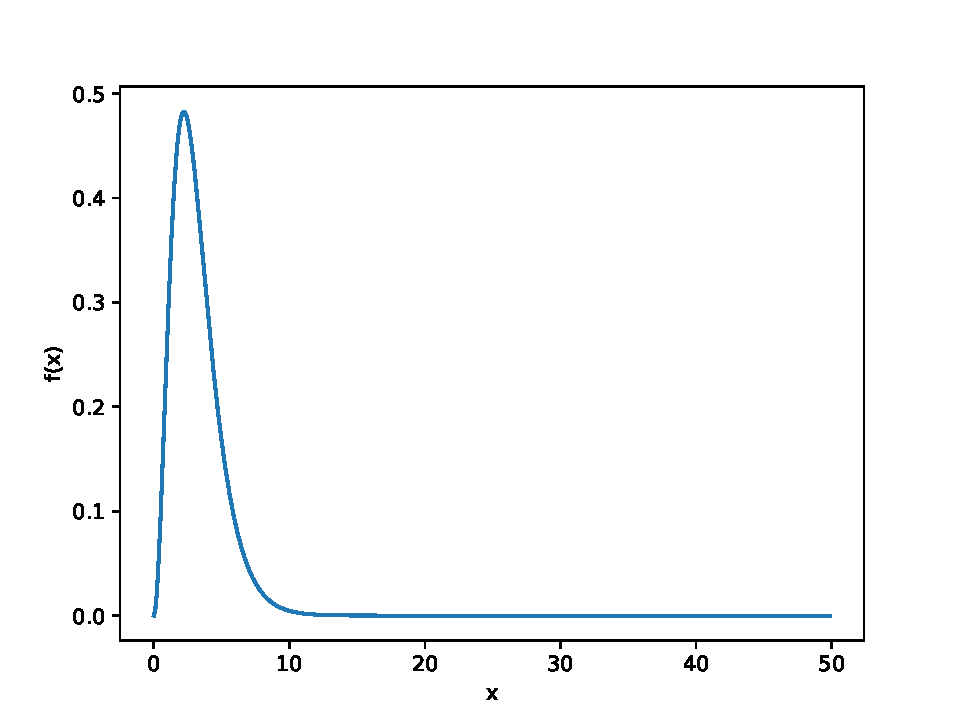
\includegraphics[scale=0.5]{plotIntegrand.pdf}
\caption{Behavior of the integrand in equation (\ref{eq:ElectronDensity}) as function of $x$.}
\label{fig:plotIntegrand}
\end{figure}

Note that values of $x>20$ give values of  $f(x)$ so small that they will not contribute greatly to the value of the integral. Hence, the infinite upper limit in the integral in equation (\ref{eq:ElectronDensity}) will be replaced by a finite value $x_{max}$, for which the value of the integrand falls below the epsilon of the machine ($ f(x_{max}) < \epsilon \sim 10^{-16}$).

In order to calculate the constant in front of the integral,
\begin{equation}
C = {8\pi (k_BT)^3 \over (2\pi\hbar
  c)^3} ,
\end{equation}
we need the values
\begin{eqnarray}
k_BT &=& 20 \text{ MeV} = 3.20435\times 10^{-12} \text{ J} \\
\hbar &=& 1.0545718 \times 10^{-34} \text{ m}^2 \text{kg/s}\\
c &=& 3 \times 10^8 \text{ m/s} ,
\end{eqnarray}
giving the result
\begin{equation}
C = 1.052756 \times 10^{41} \text{ m}^{-3}.
\end{equation}

The code in the file solution6.2a.py solves the adimensional integral using the midpoint rule with the parameter $h=1\times 10^{-5}$ and the upper limit as described above. The resulting value for the integral is
\begin{equation}
\int_0^\infty  \frac{x^2 dx}{e^{x} + 1} = 1.803085354731
\end{equation}
and the corresponding number density of electrons gives
\begin{equation}
n_{e^\pm} = 1.8982095515123674 \times 10^{41} \text{ m}^{-3}. \label{eq:electronDensity1}
\end{equation}

b) In order to write the integral in the adequate terms, remember  that the energy of the photons is $E = pc$ and therefore $x=\beta E$. Hence, the number density of electrons is written as
\begin{eqnarray}
n_{e^\pm}  &=&  {8\pi (k_BT)^3 \over (2\pi\hbar c)^3}\int_0^\infty  \frac{x^2 dx}{e^{x} + 1}\\
&=& {8\pi  \over (2\pi\hbar c)^3} \int_0^\infty  \frac{E^2 dE}{e^{\beta E} + 1}.
\end{eqnarray}

This equation let us write 
\begin{equation}
\left[ n_{e^\pm} \right]_i = {8\pi  \over (2\pi\hbar c)^3} \int_{E_i}^{E_{i+1}}  \frac{E^2 dE}{e^{\beta E} + 1}
\end{equation}
and then
\begin{equation}
\left[\frac{dn_{e^\pm}}{dE} \right]_i = \frac{[n_{e^\pm}]_i }{ \Delta E}.
\label{eq:spectrumEquation}
\end{equation}

The code in the file solution6.2b.py takes the width of the intervals as $\Delta E = E_{i+1} - E_i = 5 \text{ MeV}$ to calculate the integral. The resulting spectrum is represented in the Figure \ref{fig:plotSpectrum}, which has exactly the same form as that in Figure \ref{fig:plotIntegrand}.
\begin{figure}
\centering
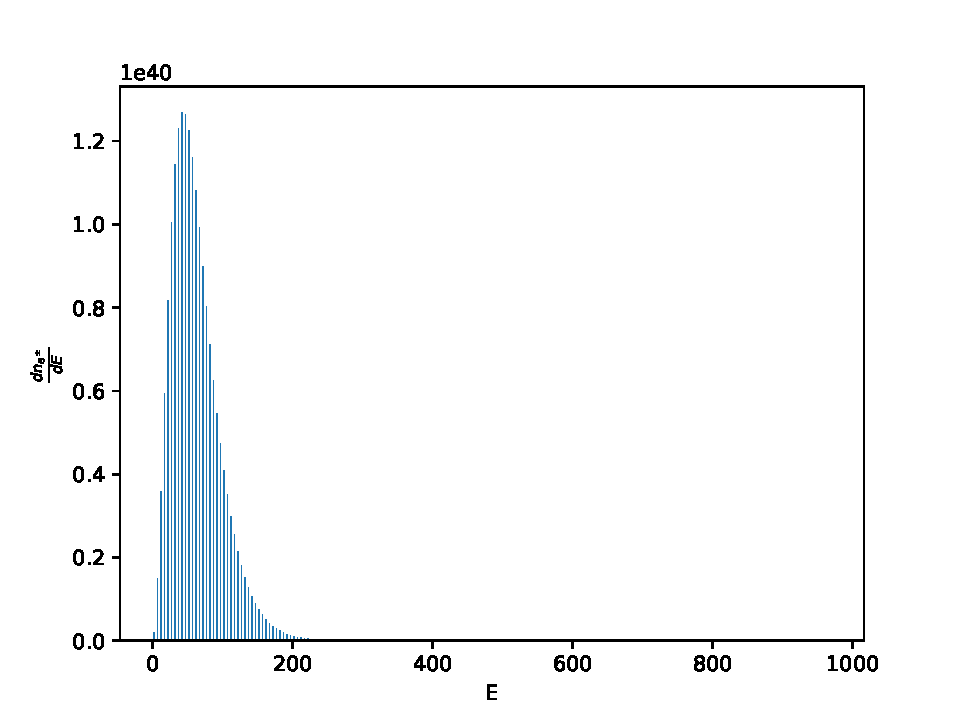
\includegraphics[scale=0.5]{plotSpectrum.pdf}
\caption{Behavior of the spectrum of electrons from equation (\ref{eq:spectrumEquation}) as function of the energy $E$.}
\label{fig:plotSpectrum}
\end{figure} 

To check our integration, the file solution6.2b.py also calculates the total density of electrons as
\begin{equation}
n_{e^\pm} = \sum_i \left[\frac{dn_{e^\pm}}{dE} \right]_i \Delta E,
\label{eq:spectrumEquation}
\end{equation}
and the result is 
\begin{equation}
n_{e^\pm} = 1.8982348403614643 \times 10^{41}  \text{ m}^{-3} \label{eq:electronDensity2}
\end{equation}
which  differs from the result in equation (\ref{eq:electronDensity1}) by a $1.3 \times 10^{-3} \ \%$ .
 




\end{document}
